\documentclass{standalone}
\usepackage{tikz}
\usetikzlibrary{arrows.meta}
\begin{document}
\usetikzlibrary{positioning}
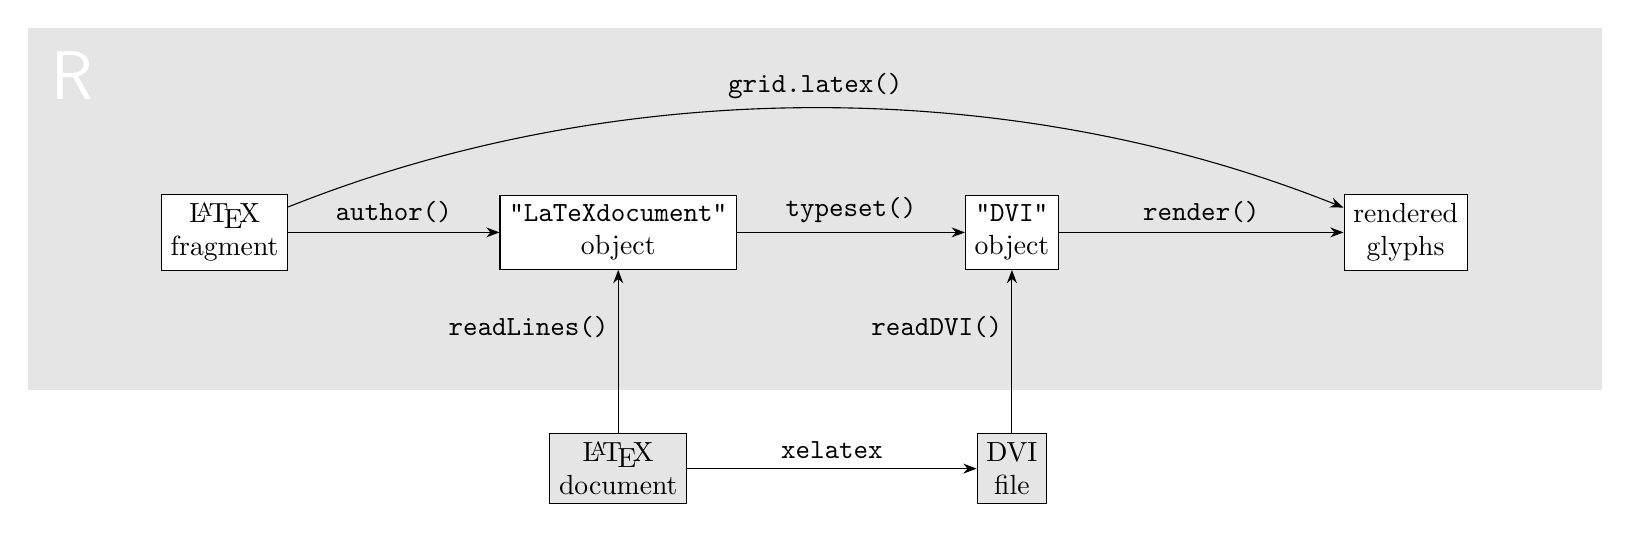
\begin{tikzpicture}[every node/.style={draw}, x=5cm, y=2cm]
  % \draw[help lines] (0,0) grid (2,3);

  \tikzset{R node/.style={rectangle,draw,fill=white,align=center}}
  \tikzset{other node/.style={rectangle,draw,fill=black!10,align=center}}
  \tikzset{horiz label/.style={draw=none,midway,above}}
  \tikzset{vert label/.style={draw=none,pos=.65,left}}

  \path[fill=black!10] (-.5, -1) rectangle (3.5, 1.3);

  \path (-.5, 1.3) 
        node[draw=none,text=white,anchor=north west,below right=5pt,font=\bfseries] 
        {\Huge {\sf R}};

  \path 
    (0, 0) node[R node](a1) {\LaTeX\\ fragment} 
    (1, 0) node[R node](b1) {{\tt "LaTeXdocument"}\\ object}
    (2, 0) node[R node](c1) {{\tt "DVI"}\\ object}
    (3, 0) node[R node](d1) {rendered\\ glyphs}
    (1, -1.5) node[other node](b2){\LaTeX\\ document}
    (2, -1.5) node[other node](c2){DVI\\ file}
  ;

  \draw[-Stealth] (a1) -- (b1) node[horiz label] {{\tt author()}};
  \draw[-Stealth] (b1) -- (c1) node[horiz label] {{\tt typeset()}};
  \draw[-Stealth] (c1) -- (d1) node[horiz label] {{\tt render()}};
  \draw[-Stealth] (b2) -- (b1) node[vert label] {{\tt readLines()}};
  \draw[-Stealth] (c2) -- (c1) node[vert label] {{\tt readDVI()}};
  \draw[-Stealth] (b2) -- (c2) node[horiz label]{{\tt xelatex}};

  \draw[-Stealth] (a1) .. controls (1, 1) and (2, 1) .. (d1) 
                  node[horiz label] {{\tt grid.latex()}};

\end{tikzpicture}
\end{document}

